
 \documentclass[answers]{exam}
 
 \usepackage{graphicx}
 \usepackage{float}
 \usepackage{amsmath}
 \usepackage{amsfonts}
 \usepackage{amsthm}
 \usepackage{framed}
 \usepackage{algorithmicx}
 \usepackage{algpseudocode}
 \newcommand{\ans}[1]{\begin{framed}{\textbf{Answer:} #1}\end{framed}}
 \newcommand{\sol}{\uplevel{\textsc{Solution:}}}
 \newenvironment{answer}{%
     \renewcommand{\solutiontitle}{\noindent\textbf{Answer:}\enspace}
     \begin{solution}
     }{%
     \end{solution}
     \renewcommand{\solutiontitle}{\noindent\textbf{Solution:}\enspace}
 }
 \newtheorem*{claim}{Claim}
 \newtheorem{lemma}{Lemma}

 
% First we setup the header and footer
\pagestyle{headandfoot}
\runningheadrule
\runningfootrule
\header{COL351: Analysis and Design of Algorithms (CSE, IITD, Semester-I-2020-21)}{}{Homework-1}
\footer{}{\thepage  \, of \numpages}{}
 
% We want the points for each question displayed on the left
%\pointname{points}
%\pointsinmargin
 
% Automatically total the points - make sure to compile TWICE
\addpoints
 
\begin{document}


\begin{center} 
\fbox{\parbox{5.5in}{
\vspace{-0.1in}
\begin{itemize}
\item \small{Please note that one of the main goals of this course is to design efficient algorithms. So, there are points for efficiency even though we may not explicitly state this in the question. }

\item \small{Unless otherwise mentioned, assume that graphs are given in adjacency list representation.}

\item \small{In the lectures, we have discussed an $O(V+E)$ algorithm for finding all the SCCs of a directed graph. We can extend this algorithm to design an algorithm {\tt CreateMetaGraph($G$)} that outputs the meta-graph of a given directed graph in $O(V+E)$ time. For this homework, you may use  {\tt CreateMetaGraph($G$)} as a sub-routine.}

\item \small{The other instructions are the same as in Homework-0.}
\end{itemize}
\vspace{-0.1in}
}}
\end{center}

\vspace{0.1in}


\vspace{0.1in}
% Some general text together with number of questions and total points possible
There are \numquestions\, questions for a total of \numpoints\, points.
\vspace{0.1in}
\hrule
 \vspace{0.2in}
\begin{questions}
 
% First question, worth 3 points
\question An undirected graph is said to be {\em connected} iff every pair of vertices in the graph are reachable from one another. Prove the following statement:
\begin{quote}
{\it Any connected undirected graph with $n$ nodes has at least $(n-1)$ edges.}
\end{quote}

We will prove the statement using Mathematical Induction. The first step in such a proof is to define the propositional function. Fortunately for this problem, this is already given in the statement of the claim. 

$P(n)$: Any connected undirected graph with $n$ nodes has at least $(n-1)$ edges.

The base case is simple. $P(1)$ holds since any connected graph with $1$ node having at least $0$ edges, is indeed true. 
For the inductive step, we assume that $P(1), P(2), ..., P(k)$ holds for an arbitrary $k \geq 1$, and then we will show that $P(k+1)$ holds. Consider any connected graph $G$ with $(k+1)$ nodes. You are asked to complete the argument by doing the following case analysis:

\begin{parts}
\part[5] Show that if the degrees of all nodes in $G$ is at least $2$, then $G$ has at least $k$ edges.

\begin{solution}
To show this we will first prove the following.

\begin{claim}
For any graph $G (V, E)$ : $\sum_{v \in V} d_v = 2 |E|$ where $d_v$ is degree of vertex $v \in V$
\end{claim}
\begin{proof}
We shall prove the claim by principle of induction.
\[
    P(n) : \text{The claim holds for all }G(V,E)\text{ such that }|E| \leq n
\]
\textbf{Base Case:} $P(0)$ is trivially true as a graph with no edges will have all zero-degree vertices.
\textbf{Induction Step:} Suppose $P(n)$ is true. Let $G(V,E)$ be any graph such that $|E|=n+1$. Pick any edge
$e \in E$ and delete it from this graph. After deleting this edge the graph will have $n$ edges and the degree
of exactly two incident vertices will decrease by 1. Since $P(n)$ holds we may write
\begin{align*}
                \sum_{v \in V} {d_v} - 2 &= 2(|E|-1)\\
    \implies    \sum_{v \in V} {d_v} &= 2|E|
\end{align*}
Thus, $P(n+1)$ is also true. Hence the induction is established and claim is proved.
\end{proof}
Now, we are given that $G$ has $k+1$ nodes all such that $d_v \geq 2$. From the claim proved above, we may therefore
write for $G$
\begin{align*}
    \sum_{v \in V} {d_v} &= 2 |E|\\
    \sum_{v \in V} {2} &\leq 2 |E|\\
    \sum_{v \in V} {1} &\leq |E|\\
    k+1 &\leq |E|
\end{align*}
Thus we have $|E| \ge k + 1 > k$, as needed.
\end{solution}

\part[5] Consider the case where there exists a node $v$ with degree $1$ in $G$. In this case, consider the graph $G'$ obtained from $G$ by removing vertex $v$ and its edge. Now use the induction assumption on $G'$ to conclude that $G$ has at least $k$ edges.

\begin{solution}
Since the removed vertex $v$ had degree 1 we conclude that $G'$ will also be connected (as $G$ is connected). Deleting a vertex of degree 1 implies reducing $|V|$ and $|E|$ by 1, so $G'$ will have $k$ nodes and $|E'| = |E|-1$. Now, from our induction hypothesis, since $P(k)$ is assumed to be true $\implies |E'| \geq k-1$. And since $|E'| = |E|-1$ we get $|E| \geq k$. Thus, $G$ has at least $k$ edges.
\end{solution}

\end{parts}

\vspace{0.3in}

\question  Consider the following directed graph and answer the questions that follow:

\begin{figure}[h]
\centering
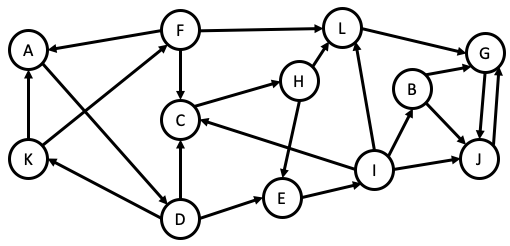
\includegraphics[scale=0.6]{scc}
\end{figure}

\begin{parts}
\part[1] Is the graph a DAG?

\begin{solution}
No; $G\to J \to G$ is a cycle.
\end{solution}

\part[2] How many SCCs does this graph have?

\begin{solution}
$5$; $\{A,D,K,F\}, \{C,E,H,I\}, \{B\}, \{L\}, \{G,J\}$.
\end{solution}

\part[1] How many source SCCs does this graph have?

\begin{solution}
$1$; $\{A,D,F,K\}$
\end{solution}

\part[2] What is the distance of node $B$ from the $A$?

\begin{solution}
$4$; corresponding shortest path: $A \to D \to E \to I \to B$.
\end{solution}

\part[2] Suppose we run the DFS algorithm on the graph exploring nodes in alphabetical order. Given this, what is the pre-number of vertex $F$?

\begin{solution}
20
\end{solution}

\part[2] Suppose we run the DFS algorithm on the graph exploring nodes in alphabetical order. Given this, what is the post-number of vertex $J$?

\begin{solution}
10
\end{solution}

\end{parts}

\vspace{0.3in}


\question[20] Suppose a degree program consists of $n$ mandatory courses.
The {\em prerequisite graph} $G$ has a node for each course, and an edge from course $u$ to course $v$ if and only if $u$ is a prerequisite for $v$. Design an algorithm that takes as input the adjacency list of the prerequisite graph $G$ and outputs the minimum number of quarters necessary to complete the program. You may assume that there is no limit on the number of courses a student can take in one quarter. 
Analyse running time and give proof of correctness of your algorithm.

\begin{solution}
The algorithm for the problem follows. We have assumed that a routine \textbf{Linearize($G$)} is already defined which takes a graph $G$ and returns a random-accessible list of vertices in G in linearized order (topologically sorted). This is exactly the algorithm discussed in class.

In the algorithm that follows, we denote by minq[v] the minimum quarter in which the course v may be completed. We shall prove, in the proof of correctness, that the algorithm correctly computes minq[v] for all courses.

Note that for a solution to even exist the prerequisite graph must be acyclic. Because a cycle in dependency implies that no course in that cycle can ever be taken. For convenience in notation, we assume that the \textbf{linearize} routine fails when given such a graph.

\begin{algorithmic}[1]
\Function{minimumQuarters}{$G$}
    \State $n \gets |V(G)|$
    \State let courses $\gets$ \Call{linearize}{$G$} \Comment{topologically sorted list of vertices}
    \If{\emph{linearize fails}} \Comment {Linearization fails \textbf{iff} $G$ is not acyclic.}
        \State \Return $\infty$  \Comment {If G has a cycle then those courses can never be completed.}
    \EndIf
    \State let minq $\gets$ array of size $n$ initialized to all 1.
    \For{$i=1 \ldots n$}
        \State $u \gets \text{courses}[i]$
        \ForAll{$v \text{\,such\,that\,} (u, v) \in E(G)$}
            \State minq$[v] = \max (\text{minq}[v], \text{minq}[u]+1)$
        \EndFor
    \EndFor
    \State \Return $\max \{minq[i]: i \in [1\ldots n]\}$ \Comment {Minimum quarters required to complete all course}
\EndFunction
\end{algorithmic}

\textbf{Proof of correctness:}
\begin{proof}
First we shall prove that the following loop-invariant holds.
\begin{align*}
    P(i): & \text{After the $i$th iteration of loop (8-12)},\\
         & \text{minq}[v] = 1 + \max \{\text{minq}[u]:\, u \in \text{courses}[1\ldots i] \;\text{and}\; \text{edge}(u, v)\} \\
         & \text{for all } v \in \text{courses}
\end{align*}
For convenience here we have assumed $\max \emptyset = 0$

\textbf{Base Case: } $P(0)$ is trivially true because minq is initialized to all 1s in line 7 before the loop.

\textbf{Inductive Step: } Let us assume $P(i-1)$ is true. We will show that this implies that $P(i)$ is also true.

Let $v$ be any course. Following cases arise -

\textbf{Case 1: } $v$ has the course courses$[i]$ as its direct pre-req.

Note that at the $i$th iteration the following update happens for all courses $v$ which have courses$[i]$ as their pre-req. (refer line 10-12 in pseudocode)
\[
    \text{minq}[v] = \max (\text{minq}[v]_{prev}, \text{minq}[\text{courses}[i]] + 1)
\]
Since $P(i-1)$ is assumed, before the i-th iteration we must have had
\[
    \text{minq}[v]_{prev} = 1 + \max \{\text{minq}[u]:\, u \in \text{courses}[1\ldots i-1] \;\text{and}\; \text{edge}(u, v)\} 
\]
Thus, substituting $\text{minq}[v]_{prev}$ in the update expression above we can finally obtain
\[
    \text{minq}[v] = 1 + \max \{\text{minq}[u]:\, u \in \text{courses}[1\ldots i] \;\text{and}\; \text{edge}(u, v)\} 
\]
Thus, $P(i)$ holds for this case.

\textbf{Case 2: } $v$ does not have the course courses$[i]$ as its direct pre-req

If courses$[i]$ is not a pre-req then there must be no edge from courses$[i]$ to v. This implies that we have $\{u:\, u \in \text{courses}[1\ldots i-1] \;\text{and}\; \text{edge}(u, v)\} = \{u:\, u \in \text{courses}[1\ldots i] \;\text{and}\; \text{edge}(u, v)\}$

Therefore, in this case also $P(n)$ holds.

Hence the induction has been established and loop-invariant holds.

Now to complete the proof all that remains is to show that at the end of loop, minq$[v]$ is the minimum quarter number in which the course $v$ may be completed if all the prerequisites are completed optimally. We shall again prove this claim by induction.

P(k): In any valid assignment of quarter numbers to courses, quarter number in which course $u$ is completed $>=$ minq$[u]$ for all $u \in \text{courses}[1\ldots k]$

\textbf{Base Case: } $P(1)$ holds because minq[courses[$1$]] is initialized to 1 and is never modified again (see loop invariant above) and since it is a source vertex (as courses is topologically sorted order) it must have no pre-requisites and therefore it can be completed in the very first quarter.

\textbf{Inductive Step: } Let us assume that $P(k-1)$ holds, we will show that this implies that $P(k)$ is also true.

Note that for any course $u$ it can never be taken before all its pre-requisite courses have been completed. Thus, we can write
\[
    \text{quarter for course }u \geq 1 + \max\{\text{quarter for course }v : v \in \text{courses} \;and\; \text{edge}(v,u)\}
\]
Now we observe that it is always possible to take this course $u$ in the very next quarter once all its pre-requisite courses have been completed. Therefore the lower-bound of minimum quarter number as shown above is achievable.

Because courses is a linearized list of vertices of G we have that : all pre-requisite courses of courses[$k$] belong to $\text{courses}[1\ldots k-1]$. Therefore we have
\[
    \{v:\, v \in \text{courses}[1\ldots k-1] \;and\; \text{edge}(v,\text{courses}[k])\} = \{v:\, v \in \text{courses} \;and\; \text{edge}(v,\text{courses}[k])\}
\]
and thus,
\begin{align*}
    \text{quarter for courses[k]} \geq 1 + \max\{&\text{quarter for course }v :\\
                                                     &v \in \text{courses}[1\ldots k-1] \;and\; \text{edge}(v,\text{courses}[k])\}
\end{align*}
Now, since we assumed $P(k-1)$ we have that minq$[v]$ store the respective lower bound values for all courses $v \in \text{courses}[1\ldots k-1]$. We finally have,
\[
    \text{quarter for course[k]} \geq 1 + \max\{\text{minq}[v] : v \in \text{courses}[1\ldots k-1] \;and\; \text{edge}(v,\text{courses}[k])\}
\]
which is exactly minq[courses[$k$]] from loop invariant established before.

Therefore induction is established and hence the proof is complete.

Now we will show one optimal strategy to complete the courses in minimum quarter numbers. The strategy is very simple, we complete every course $u$ in its respective $minq[u]$ quarter. This is a valid assignment because such an assignment guarantees that a course is never taken before all of its pre-requisites have been completed, and it is always possible to take the course the very next quarter after its pre-requisites have been completed because we are given that we may do as many courses as possible in a quarter. This strategy is optimal simply because quarter numbers for each course have a lower bound as shown in previous induction and in this strategy the lower bound is achieved for each course. So our final answer will be max(minq) because we have to keep completing courses till all the courses have been completed.
\end{proof}

\textbf{Running Time Complexity: }

The \textbf{linearize} routine is supposed to be implemented as done in class in $O(|V|+|E|)$ running time. minq is also an array of size $|V|$ therefore initializing it will take further $O(|V|)$ steps. The outer loop performs exactly $V$ iterations and the inner loop performs exactly $d_{\text{courses}[i]}$ iterations where $d_v$ denotes out-degree of vertex $v$. Therefore the total number of iterations performed are $\sum_{v \in \text{courses}} d_v = |E|$. Note that because $G$ is given in adjacency list representation the inner loop in pseudocode may be directly implemented by iterating adjacency list associated with the respective course. In each iteration 2 memory accesses and a maximum operation and an addition operation is performed. Each operation will take $O(1)$ steps assuming arrays are random-accessible.

Finally, we take max of the entire minq array which will further take $O(|V|)$ steps. For space requirements we have 2 arrays : courses and minq each of size exactly $|V|$. So, in conclusion, the analysis yields -
\[
    \text{Time Complexity: } O (|V| + |E|)
\]
\end{solution}

\vspace{0.3in}

\question A particular  video game involves walking along some path in a map that can be represented as a directed graph $G = (V, E)$. 
At every node in the graph, there is a single bag of coins that can be collected on visiting that node for the first time. 
The amount of money in the bag at node $v$ is given by $c(v) > 0$.
The goal is to find what is the maximum amount of money that you can collect if you start walking from a given node $s \in V$.
The path along which you travel need not be a simple path. 

Design an algorithm for this problem. You are given a directed graph $G = (V, E)$ in adjacency list representation and a start node $s \in V$ as input. 
Also given as input is a matrix $C$, where $C[u] = c(u)$.
Your algorithm should return the maximum amount of money that is possible to collect when starting from $s$.
\begin{parts}
\part[10] Give a linear time algorithm that works for DAG's.

\begin{solution}
We have assumed that a routine $\textbf{Linearize(G)}$ is already defined which takes Graph $G$ and returns a random accesible list of vertices in $G$ in linearized order(topologically sorted). This is exactly the algorithm discussed in class.

In the algorithm that follow we have denoted maxcoins[v] as the maximum number of coins that can be collected if you start walking from s(starting node) and end your journey at node v. We will prove, in the proof of correctness that the algorithm correctly computes maxcoins[v] for all nodes.

\begin{algorithmic}[1]
\Function{maximumMoney}{$G, C$}
     \State $n \gets V(G)$
     \State let toponodes $\gets$ \Call{Linearize}{$G$}   \Comment{topologically sorted list of nodes}
     \State let maxcoins $\gets$ array of size n initialized to all 0
     \State maxcoins$[s] \gets $C$[s]$
     \State let $i_{1}$ $\gets$ index of s in toponodes
     \For{$i=i_{1} \ldots n$}
        \State $u \gets$ toponodes[$i$]
        \ForAll{$v$ such that $(u,v) \in E(G)$}
            \State maxcoins[$v$] $\gets$ max(maxcoins[$v$], C[$v$]+maxcoins[$u$])
        \EndFor
    \EndFor 
    \State \Return $\max\{\text{maxcoins}[i]:i \in [1\ldots n]\}$ \Comment{Maximum amount of money can be collected}
\EndFunction
\end{algorithmic}
\textbf{Proof of correctness}
\begin{proof}
First we will prove this claim.

\textbf{Claim:} For all v $\in$ toponodes\{1,...$i_{1}$-1\} maxcoins[v]=0.

\begin{proof}
As all these nodes come before $s$ in topological order $\implies$ there is no path from $s$ to these nodes. Therefore maxcoins$[v]=0$ for all these nodes and as the player will never reach on these nodes therefore these nodes and the edges from these nodes can be ignored in the problem and hence in our proof.
\end{proof}

maxcoins$[s]=C[s]$ As it will collect coins of only that node if it finish at $s$ itself.

Now we shall prove that the following loop-invariant holds.
\begin{align*}
    P(k): & \text{After the $k$th iteration of loop (7-12)},\\
          & \text{maxcoins}[v] =  \max \{C[v]+\text{maxcoins}[u]:\, u \in \text{toponode}[i_{1}\ldots i_{1}+k-1] \;\text{and}\; \text{edge}(u, v)\} \\
          & \text{for all } v \in \text{toponodes}[i_{1}+1 \ldots n]
\end{align*}

\textbf{Base Case:} $P(0)$ is true trivially because maxcoins is initialized to all 0s in line4 before the loop using the above proved claim.

\textbf{Inductive Step:} Let us assume $P(k)$ is true. We will show that this implies that $P(k+1)$ is also true.

\textbf{Case 1:} $v$ has direct edge with node toponodes$[k+i_{1}]$ .

Note that at the $(k+1)$th iteration the following update happens for all nodes $v$ which have edge with toponodes$[k+i_{1}]$. (refer line 9-11 in pseudocode)
\[
    \text{maxcoins}[v] = \max (\text{maxcoins}[v]_{prev}, \text{maxcoins}[\text{toponodes}[k+i_{1}]] + C[v])
\]
Since $P(k)$ is assumed, before this (k+1)-th iteration we must have had
\[
    \text{maxcoins}[v]_{prev} = \max \{C[v] + \text{maxcoins}[u]:\, u \in \text{toponodes}[i_1\ldots i_{1}+k-1] \;\text{and}\; \text{edge}(u, v)\} 
\]
Thus, substituting $\text{maxcoins}[v]_{prev}$ in the update expression above we can finally obtain
\[
    \text{maxcoins}[v] = \max \{C[v] + \text{maxcoins}[u]:\, u \in \text{toponodes}[i_1\dots k+i_{1}] \;\text{and}\; \text{edge}(u, v)\} 
\]
Thus, $P(k+1)$ holds for this case.

\textbf{Case 2: } $v$ does not have the edge from node toponodes$[k+i_{1}]$ 

If there is no edge from toponodes$[k+i_{1}]$ to v. Then this implies that we have $\{u:\, u \in \text{toponodes}[i_1\ldots k+i_{1}-1] \;\text{and}\; \text{edge}(u, v)\} = \{u:\, u \in \text{toponodes}[i_1\ldots k+i_{1}] \;\text{and}\; \text{edge}(u, v)\}$

Therefore, in this case also $P(k+1)$ holds.

Hence the induction is established and loop invariant holds.

Now to complete the proof all that remains is to show that at the end of loop, maxcoins[v] is the maximum amount of money which can be collected if the player starts at node s and ends his journey at node v.  We shall again prove this claim by induction.
\begin{align*}
    P(k):& \text{maxcoins}[u] \text{ stores the maximum amount of money which can be collected} \\
         & \text{if player starts at node $s$ and ends his journey at $u$},\; u \in \text{toponodes}[i_{1}\ldots k+i_{1}]
\end{align*}
\textbf{Base Case:} $P(0)$ holds because maxcoins[toponodes[$s$]] = maxcoins[toponodes[$i_{1}$]] is initialized to $C[s]$ and since it is a starting vertex and the graph is DAG it can never be modified again in the loop.

\textbf{Inductive Step:} Let us assume that $P(k-1)$ holds, we will show that this implies that $P(k)$ is also true.

Note that for any node the maximum amount of money collected till it will be the sum of c[u]+ maximum money collected till one of its predecessor in toponodes$[i_1 \ldots n]$. We may write this mathematically as -
\[
    \text{maximum money till }u = \max\{C[u] + \text{maximum money till }v : v \in \text{toponodes} \;and\; \text{edge}(v,u)\}
\]

Because toponodes is a topologically sorted list of vertices of G we have that : all nodes from which there is an edge to toponodes[$k+i_{1}$] belong to $\text{toponodes}[i_{1}\ldots k+i_{1}-1]$. Therefore we have
\begin{align*}
    &\{v:\, v \in \text{toponodes}[i_{1}\ldots k+i_{1}-1] \;and\; \text{edge}(v,\text{toponodes}[k+i_1])\} \\ & =
    \{v:\, v \in \text{toponodes}[i_1\ldots n] \;and\; \text{edge}(v,\text{toponodes}[k+i_1]))\}
\end{align*}
and thus,
\begin{align*}
    &\text{maximum money till toponodes}[k+i_{1}] \\&= \max\{C[\text{toponodes}[k+i_{1}]]+\text{maximum money till }v :\\&
                                v \in \text{toponodes}[i_{1}\ldots k+i_{1}-1] \;and\; \text{edge}(v,k+i_{1})\}
\end{align*}
Now, since we assumed $P(k-1)$ we have that maxcoins$[v]$ store the respective maximum values for all nodes $v \in \text{toponodes}[i_{1}\ldots k+i_{1}-1]$. We finally have,
\begin{align*}
    &\text{maximum money till toponodes}[k+i_{1}] \\&= \max\{C[\text{toponodes}[k+i_{1}]]+ \text{maxcoins}[v] :
                                            \\&v \in \text{toponodes}[i_{1}\ldots k+i_{1}-1] \;and\; \text{edge}(v,\text{toponodes}[k+i_{1}])\}
\end{align*}
which is exactly maxcoins[toponodes[$k+i_{1}$]] from loop invariant established before.

Therefore induction is established and hence the proof is complete.

Now that we have proved that maxcoins[$v$] is equal to the maximum money that can be collected when we start our journey at s and ends at v, so the answer to the problem is simply max(maxcoins), i.e., the maximum of all elements in the array maxcoins.

\end{proof}

\textbf{Running Time Complexity: }

The \textbf{linearize} routine is supposed to be implemented as done in class in $O(|V|+|E|)$ running time. maxcoins is also an array of size $|V|$ therefore initializing it will take further $O(|V|)$ steps. Finding the index of s in toponodes will also take $O(|V|)$ steps. The outer loop performs exactly $|V|$ iterations and the inner loop performs exactly $d_{\text{toponodes}[i]}$ iterations where $d_v$ denotes out-degree of vertex $v$. Therefore the total number of iterations performed are $|V| + \sum_{v \in \text{nodes}} d_v = |V| + |E|$ In each iteration 2 memory accesses and a maximum operation and an addition operation is performed. Each operation will take $O(1)$ steps assuming arrays are random-accessible.

Finally, we take max of the entire maxcoins array which will further take $O(|V|$) steps. For space requirements we have 2 arrays : toponodes and maxcoins each of size exactly $|V|$. So, in conclusion, the analysis yields -
\[
    \text{Time Complexity: } O (|V| + |E|)
\]


\end{solution}

\part[10] Extend this to a linear time algorithm that works for any directed graph.
({\it \underline{Hint}: Consider making use of the meta-graph of the given graph.})

\begin{solution}
Consider the meta-graph $G^M$ of the graph $G$. We will first prove a number of useful lemmas and gradually build towards the final proof.\\

\begin{lemma}
Firstly, we show that there is a path from $u$ to $v$ in $G$ iff there is a path from $Component(u)$ to $Component(v)$ in $G^M$.
\end{lemma}

\begin{proof}
Proving the iff by proving from both sides -

\textbf{Part 1:} (Path from $u$ to $v$ $\implies$ path from $Component(u)$ to $Component(v)$ in $G^M$)

Suppose the path from $u$ to $v$ in $G$ is $u = v_1, v_2, ..., v_n = v$. Then since there is an edge from $v_i$ to $v_{i + 1}$, either they are in the same component or there is an edge from $Component(v_i)$ to $Component(v_{i + 1})$. So if we consider the sequence $$Component(u) = Component(v_1), Component(v_2) ..., Component(v_n) = Component(v)$$ and remove adjacent equal components, then this is a path from $Component(u)$ to $Component(v)$ in $G^M$.

\textbf{Part 2:} (Path from $Component(u)$ to $Component(v)$ in $G^M$ $\implies$ path from $u$ to $v$)

Suppose the path from $Component(u)$ to $Component(v)$ in $G^M$ is $$Component(u) = Component_1, Component_2, \dots, Component_n = Component(v)$$ Suppose an edge connecting a vertex in $Component_i$ to one in $Component_{i + 1}$ is $(v_i, v_i')$. Also define $v_0' = u$ and $v_n = v$. 
Let the path $p_{ij}$ be the path from vertex $i$ to vertex $j$.

Then the path $$\left(\bigcup_{i = 0}^{n - 2} p_{v_i'v_{i + 1}}\cup \{(v_{i + 1}, v_{i + 1}')\}\right) \cup p_{v_{n - 1}'v_{n}}$$ is a valid path from $u$ to $v$, where the union symbol is used to join paths with a common endpoint and same orientation (for a more verbose explanation of this formula, please see the solution to problem 5b).
\end{proof}

%Since we are done with both parts, we have shown that we can focus our attention to the meta-graph of a graph; in particular, it means that we can safely work with only DAGs.

% change claim to a stronger condition, that for any node u on the best path, SCC of u has already been visited in it.

\begin{lemma}
For any vertex $v$ on the best path from $u$ to any vertex, any vertex in the SCC of $v$ is also on the path.
\end{lemma}

\begin{proof}
Suppose there is a vertex $v'$ in the SCC of $v$ that is not in the best path. Since $v, v'$ are in the same SCC, there is a path from $v$ to $v'$ and from $v'$ to $v$. Now consider adding these paths in the best path when we reach $v$. Then we have added at least $c(v')$ coins to the best path, which is a contradiction to the optimality of the best path.
\end{proof}

The above lemma proves that it is optimal to visit all vertices in a SCC if we visit even one vertex in that SCC. Thus we may define from here onwards $C':\,C'[SCC]=\sum_{v \in SCC} C[v]$

For any SCC $Comp$ and vertices $v, u$ in it, let us define $Trav_2(S, u, v)$ as the path from $u$ to $v$ in $Comp$. Let us also define
\[
Trav(S, u) = \bigcup_{v \in Comp} Trav_2(S, u, v) \cup Trav_2(S, v, u)
\]
Here again the union symbol is used for joining two paths. Note that by traversing $Trav(S, u)$, we can traverse the whole component $Comp$ and return back to $u$.

Now, we are ready to tackle the final claim.\\

\begin{claim}
We can apply the algorithm in problem 4a on metagraph $G^M$ (considering the SCCs as a single node and number of coins of components stored in $C'$ as described in the beginning) to solve the problem for the graph $G$.
\end{claim}

%For this we need to show that the best path in $G$ can be found from the best path in $G^M$.

To show this, we show that there is an optimal path in $G$ induced by an optimal path in $G^M$.

\begin{proof}
Suppose $P: Component(s) = Component_1, Component_2, ..., Component_k$ is an optimal path in $G^M$. Then if $Component_i$ is joined to $Component_{i + 1}$ with the edge $(u_i, u_i')$ with $u_i \in Component_i$ and $u_i' \in Component_{i + 1}$, consider the following path:
\begin{align*}
P_G&: Trav(Component_1, s) \cup Trav_2(Component_1, s, u_1)\\
    & \cup \{(u_1, u_1')\} \cup Trav(Component_2, u_1') \cup Trav_2(Component_2, u_1', u_2) \cup \dots \\
    & \cup \{(u_{n - 1}, u_{n - 1}')\} \cup Trav(Component_n, u_{n - 1}') \cup Trav_2(Component_n, u_{n - 1}', v)
\end{align*}

All we now need to show is that $P_G$ is an optimal path in $G$. To show this, suppose there is a better path which visits a vertex $x$ not in these vertices. Since $Trav$ visits all vertices of a component, $x$ is not in any of the components in $P$.

Suppose the better path is $P': s, v_1', \dots, v_m'$.

Then we claim that the path $P'': Component(s), Component(v_1'), ..., Component(v_m')$ is a path with a larger number of coins than $P$, which will lead to a contradiction (here in the exhibited walk, we remove adjacent duplicates, hence this is a valid walk).

For the sake of convenience, call the number of coins at a vertex the \textbf{cost} of the vertex.

The cost of $P$ in $G^M$ is the sum of costs of all the vertices in all components covered by it (by definition of the cost of a component as the sum of costs of each vertices). Also, the path induced by it in $G$ has the same cost, since we visit all the nodes in each component (and we visit only those nodes which belong to at least one component in $P$).

Now note that the vertices covered at least once in $P'$ are a subset of those in all components in $P''$, so $cost(P'') \ge cost(P') > cost(P_G) = cost(P)$, which contradicts the fact that $P$ is the best path in $G^M$.

Thus, we have shown that an optimal path in $G^M$ induces an optimal path in $G$ (which in fact has the same cost), and hence finding the optimal cost in $G$ is equivalent to finding the optimal cost in $G^M$, which can be done by problem 4a, as needed.
\end{proof}


% \textbf{Claim:} maxcoins($C_{u}$) has already collected the coins of every node in the SCC $C_{u}$

% Proof: Suppose this is not true and there is a node u such that the coins of that nodes are not collected and we are currently at node v.

% Then we can simply go from v to u and come back to v.

% $maxcoins($C_{u}$)_{new}=maxcoins($C_{u}$)_{prev}+c[u]$

% This contradicts our definition of maxcoins($C_{u}$) therfore the assumption was wrong.

% Let C'[$C_{u}$]=sum of all c[u] where u $\in$ edges in SCC $C_{u}$

% \textbf{Claim:} The best path in the graph G can be considered as path from components as nodes with the C' defined above.

% Proof: We have shown above that the if there is path from u to v then there is path form $C_{u}$ to $C_{v}$. 

% We have also shown that before leaving the component you should have already collected all the coins in that component.

% Now we have to just show that the C' is analogous to C which we can show by showing difference between max number of coins collected before entering the component and after leaving the component is equal to sum of coins of all the nodes in that component.

% After leaving the component once you cannont come back to it again as metagraph is DAG of the SCC.

% So this means you cannot enter the same component again. and will enter the component once and leave once.

% Before entering the component you have not collected any of the coins in the component as it is your first time entering the component.

% Just before leaving you have collected all the coins in the component in the optimal path as shown above therfore the difference between the max number of coins collected before entering the component and after leaving the component is equal to sum of coins of all the nodes in that component.

% Thus prooves our claim.

% need to add up costs in the metagraph function (augment CreateMetaGraph to also merge costs)





\begin{algorithmic}[1]
\Function{maximumMoney2}{$G, C$}
    \State let $G' \gets$ \Call{CreateMetaGraph}{$G$}
    \State Initialise an array $C'$ of size $|V(G')|$ to all $0$.
    \For{each component $A$}
        \For{each vertex $v \in A$}
            \State $C'[A] \gets C'[A] + C[v]$
        \EndFor
    \EndFor
    \Comment{$C'$ as defined above}
    \State return \Call{maximumMoney}{$G', C'$}
\EndFunction
\end{algorithmic}


\textbf{Running Time Complexity: }

Creating of metagraph take $O(|V| + |E|)$. Computing of $C'$ values for all components takes $O(|V|)$ (both initialization and the computation since $|V(G')| \le |V|$ and each vertex belongs to exactly one component) and the call to problem4a's solution takes $O(|V(G')| + |E(G')|) \in O(|V| + |E|)$. Therefore
\[
    \text{Time Complexity: } O (|V| + |E|)
\]

\end{solution}
\end{parts}
Give running time analysis and proof of correctness for both parts.











\vspace{0.3in}













\question Given a directed graph $G = (V, E)$ that is not a strongly connected graph, you have to determine if there exists a pair of vertices $u, v \in V$ such that the graph $G' = (V, E \cup \{(u, v)\})$ is strongly connected. In other words, you have to determine whether there exists a pair of vertices $u, v \in V$ such that adding a directed edge from $u$ to $v$ in $G$ converts it into a strongly connected graph. Design an algorithm for this problem. Your algorithm should output ``yes'' if such an edge exists and ``no'' otherwise.
\begin{parts}
\part[10] Give a linear time algorithm that works for DAG's.

\begin{solution}

\textbf{Analysis of problem}:

Note that the graph has at least one source and one sink (as the graph is not empty, since the empty graph is vacuously strongly connected). Now we make three cases:

\begin{enumerate}
    \item The graph has at least two source nodes $s_1, s_2$. Here we make a few cases based on the endpoints of the new edge. 
    
    \begin{enumerate}
    
        \item The new edge goes from $s_i$ to $s_{3 - i}$ for some $i \in \{1, 2\}$. In this case, we do not have a path from $s_{3 - i}$ to $s_{i}$ since $s_i$ still has indegree 0.
        \item The new edge goes from any other vertex to $s_i$ for some $i \in \{1, 2\}$. In this case, we still have the indegree of $s_{3 - i}$ as 0, so there is no path from $s_i$ to $s_{3 - i}$.
        \item The new edge goes from $s_i$ to any other vertex for some $i \in \{1, 2\}$. In this case, the indegrees of $s_i, s_{3 - i}$ are still both 0, and hence there is no path from $s_i$ to $s_{3 - i}$.
        \item The new edge is not incident on any of $s_1, s_2$. In this case, the indegrees of $s_1, s_2$ are still both 0, and hence there is no path from $s_1$ to $s_2$.
    \end{enumerate}
    
    From this, we can see that this graph can never become strongly connected by the addition of just one edge.
    
    \item The graph has at least two sink nodes $s_1, s_2$. We again show that this graph can never become strongly connected by the addition of just one edge, using the analysis of the previous case. (It is possible to make 4 analogous cases for this part as well, however we won't be doing that).
    
    Suppose, for the sake of contradiction, it was possible to add an edge $(u, v)$ to $G$ to make it strongly connected. Then the reverse graph of the new graph $G' = (V, E \cup (u, v))$ is also strongly connected. However, the resulting reverse graph is the reverse of the original graph (say $G^R$) with an extra edge $(v, u)$. Since the outdegree of $s_1, s_2$ in $G$ is $0$, the indegree of $s_1, s_2$ in $G^R$ is $0$, hence they are two distinct source nodes in $G^R$. However, by our assumption, it is possible to add an extra edge to $G^R$ (which has two sources) to make it strongly connected, which is impossible by part 1, which is a contradiction to the assumption.
    
    Thus we have shown that this graph can never become strongly connected by the addition of just one edge.
    
    \item The graph has exactly one source node (say $s$) and one sink node (say $t$).
    
    \begin{claim}[\textbf{1}]Each node $v$ is reachable from the source $s$ in the original graph.
    \end{claim}
    \begin{proof} Consider the longest simple path $p$ in $G$ which contains $v$. We show that the first vertex on this path is a source node, and hence equals $s$ (which implies the claim). Suppose the first vertex $s_v$ on this path is not a source. Then it has non-zero indegree, so there is a vertex $s_v'$ such that $(s_v', s_v)$ is an edge. Clearly $s_v'$ is not on $p$, else there would be a cycle in $G$, which is given to us as a DAG. Thus we can extend the path $p$ by $s_v'$ in the backward direction, to get a longer path, which is a contradiction to the maximality of the length of $p$. Thus, $s_v$ is a source node. Since it is a source node, and $G$ has only one source, namely $s$, we have $s_v = s$, and thus $v$ is reachable from $s$, as needed.
    \end{proof}
    \begin{claim}[\textbf{2}] The sink $t$ is reachable from each node $v$ in the original graph.
    \end{claim}
    \begin{proof} This proof is completely analogous to the proof of the previous part. Consider the longest simple path $p$ in $G$ which contains $v$. We show that the last vertex on this path is a sink node, and hence equals $t$ (which implies the claim). Suppose the last vertex $t_v$ on this path is not a sink. Then it has non-zero outdegree, so there is a vertex $t_v'$ such that $(t_v, t_v')$ is an edge. Clearly $t_v'$ is not on $p$, else there would be a cycle in $G$, which is given to us as a DAG. Thus we can extend the path $p$ by $t_v'$ in the forward direction, to get a longer path, which is a contradiction to the maximality of the length of $p$. Thus, $t_v$ is a sink node. Since it is a sink node, and $G$ has only one sink, namely $t$, we have $t_v = t$, and thus $t$ is reachable from $v$, as needed.
    \end{proof}
    \begin{claim}[\textbf{3}] It is possible to add an edge to make the graph strongly connected.
    \end{claim}
    \begin{proof}
    More specifically, we shall add an edge $(t, s)$. 
    
    First we show that our choice is valid, i.e., $s \ne t$. Suppose that $s = t$. Then $s$ has both indegree and outdegree $0$, so $s$ is isolated. By the first claim above, the graph consists of only one vertex, and hence is strongly connected, which is a contradiction to the conditions given to us.
    
    To show that the graph becomes strongly connected, we show that any node $v$ is in the same strongly connected component as $s$.
    
    By our previous claims, we know $v$ is reachable from $s$, and $t$ is reachable from $v$. So we have that $t$ is reachable from $s$. Note that by the introduction of an edge from $t$ to $s$, $s$ is reachable from $t$. Hence, $s$ and $t$ are in the same strongly connected component. Also note that since $s$ is reachable from $t$ and $t$ is reachable from $v$, $s$ is reachable from $v$. However, as we have noted earlier, $v$ is reachable from $s$. Thus, $s$ and $v$ are in the same strongly connected component.
    
    Since our node $v$ was arbitrary, all nodes in the graph are in the same strongly connected component as $s$, which implies that the graph is strongly connected.
    \end{proof}
    
\end{enumerate}

From this analysis, we note that $G$ satisfies the problem conditions if and only if $G$ has exactly one source and one sink node. So we only need to check if there is exactly one source node and one sink node in $G$.\\

\textbf{Algorithm}:

\begin{algorithmic}[1]

\Procedure{Problem5a}{Directed Acyclic Graph $G = (V, E)$}
\State Initialise integer arrays $deg_{in}$[$V$], $deg_{out}$[$V$] to $0$.

\For{$u \in V$}
\For{$v \text{ such that } (u, v) \in E$}
\State $deg_{in} \left[ v \right] \gets deg_{in} \left[ v \right] + 1$
\State $deg_{out} \left[ u \right] \gets deg_{out} \left[ u \right] + 1$
\EndFor
\EndFor

\State \textbf{let} $sources \gets 0$
\State \textbf{let} $sinks \gets 0$
\For{$v \in V$}
\If{$deg_{in} \left[ v \right] == 0$}
\State $sources \gets sources + 1$
\EndIf
\If{$deg_{out} \left[ v \right] == 0$}
\State $sinks \gets sinks + 1$
\EndIf
\EndFor
\If{$sources == 1$ and $sinks == 1$}
\State Output ``yes"
\Else
\State Output ``no"
\EndIf
\EndProcedure
\end{algorithmic}

\textbf{Proof of correctness:}

Note that from our analysis, we reduced the problem to checking whether the graph has exactly one source and one sink node. 

We firstly claim that after the first loop (over all the edges), for all $v \in V$, $deg_{in}[v]$ is the indegree of $v$, and analogously, $deg_{out}[v]$ is the outdegree of $v$. For a proof, note that for each edge which has $v$ as a starting node, we increment $deg_{out}\left[v\right]$ by $1$, and for each edge which has $v$ as the ending node, we increment $deg_{in}\left[v\right]$ by $1$, so $deg_{out}\left[v\right]$ is the number of outgoing edges from $v$, which is the outdegree of $v$, and similarly, $deg_{in}\left[v\right]$ is the number of incoming edges into $v$, which is the indegree of $v$.

Now note that we increment $sources$ by $1$ if and only if the indegree is $0$, so $sources$ is the number of nodes in the graph which have indegree $0$. By the definition of a source, $sources$ is indeed the number of sources in a graph.

Similarly, $sinks$ is the number of sinks in the graph.

The proof of the final check has already been done in the analysis.\\

\textbf{Time complexity:}

Initializing the arrays takes $O(|V|)$ time.

Since we iterate over the adjacency lists for each vertex exactly once in the first loop, doing $O(1)$ work per iteration in the inner loop, and hence $O(1 + outdegree(v))$ work in the outer loop, the time complexity of the first loop is $O(|V| + |E|)$.

Since we iterate over all the vertices once in the second loop, doing $O(1)$ work in each iteration, so the time complexity of the second loop is $O(|V|)$.
Then we do $O(1)$ work in the check and the output.
This means that the final complexity is $O(|V| + |E|)$.
\[
    \text{Time Complexity: } O (|V| + |E|)
\]
\end{solution}

\part[10] Extend this to a linear time algorithm that works for any directed graph.
({\it \underline{Hint}: Consider making use of the meta-graph of the given graph.})
\begin{solution}

\textbf{Analysis of problem:}

Consider the meta-graph $G^M$ of the graph $G$. In what follows, $C(u)$ denotes the component of the vertex $u$ in $G$. We claim the following.\\

\begin{claim}$G$ satisfies problem conditions if and only if $G^M$ satisfies the problem conditions.\end{claim}

\begin{proof} We prove this by showing both sides of the implication.\\

\textbf{Part 1:} ($G$ satisfies problem conditions $\implies$ $G^M$ satisfies problem conditions)

\begin{proof}
Let the edge we add to $G$ to make it strongly connected be $(u, v)$.

Firstly we show that there is no path from $u$ to $v$ in $G$. Suppose that there was a path from $u$ to $v$ in $G$ already, which was not a direct edge. Suppose $w, z$ is a pair of vertices in $G'$ such that $z$ is not reachable from $w$ in $G$ (i.e., after we remove the edge $(u, v)$ from $G'$ to get back $G$). Then if we consider the walk $p$ formed by the path from $w$ to $u$, the old path from $u$ to $v$ (in $G$) and the path from $v$ to $z$, then we get that $z$ was already reachable from $w$ before the addition, which is a contradiction.

So $u$ and $v$ are in different strongly connected components of $G$, and thus correspond to different nodes in $G^M$. Now consider any two nodes $n_1, n_2$ in $G'' = (V(G^M), E(G^M) \cup \{(C(u), C(v))\})$, where $C$ is the mapping from the vertices to their strongly connected components. Take any vertex $v_1$ in the strongly connected component $n_1$ and $v_2$ in the strongly connected component $n_2$. Since there is a path from $v_1$ to $v_2$ in $G'$ (i.e., after the addition of the new edge), there is a path from $n_1$ to $n_2$ in $G''$. Similarly, there is a path from $n_2$ to $n_1$ in $G''$. Thus $G''$ is strongly connected, and thus adding one edge makes $G^M$ strongly connected (which it wasn't before, due to it being a DAG with at least 2 vertices, is because of $G$ not being strongly connected).

Thus we have proved Part 1.
\end{proof}

\textbf{Part 2:} ($G^M$ satisfies problem conditions $\implies$ $G$ satisfies problem conditions)

\begin{proof}
Firstly since $G^M$ is not strongly connected, it is not a singleton DAG, hence $G$ is also not strongly connected.

Suppose we add an edge $(n_1, n_2)$ to $G^M$ to get $G''$. Consider any vertices $u \in n_1$ and $v \in n_2$. Then add an edge $(u, v)$ in $G$ to get $G'$. We claim that $G'$ is strongly connected.

Consider any vertices $v_1, v_2$ in $G'$ which are in components $N_1', N_2'$ in $G^M$. If $N_1' = N_2'$ then we are done by the definition of strong connected-ness. Since $G''$ is strongly connected, there must be a path from $N_1'$ to $N_2'$. Thus, there exist components $n_2', ..., n_k'$ such that $N_1' = n_1', n_2', ..., n_k', N_2' = n_{k + 1}'$ is a path. Suppose the edge linking $n_r'$ and $n_{r+1}'$ is $(u_r, u_r')$. Note that when $n_r' = n_1$ and $n_{r + 1}' = n_2$, then $(u_r, u_r') = (u, v)$, and otherwise it is as in $G$. Let $u_0 = v_1$ and $u_{k + 1}' = v_2$. Then we have paths between $u_r'$ and $u_{r + 1}$ due to them being in the same component. Taking the union of all these paths with all the linking edges (and joining them at the common vertices), we have a path from $v_1$ to $v_2$ (for a more formal expression for this path, see solution to problem 6). (Similarly, we have a walk from $v_2$ to $v_1$). Thus $v_1, v_2$ are strongly connected.

Since $v_1, v_2$ were arbitrary, $G'$ is strongly connected, as needed for Part 2.
\end{proof}

Now that both parts have been proved, our claim is proved.
\end{proof}

Hence, for a general graph $G$, we simply need to apply the algorithm in the previous part for the meta-graph of $G$.\\

\textbf{Algorithm:}

\begin{algorithmic}[1]
\Procedure{Problem5b}{Directed Graph $G = (V, E)$}
\State \textbf{let} $G^M \gets \mathtt{CreateMetaGraph}(G)$
\State \Call{Problem5a}{$G^M$}
\EndProcedure
\end{algorithmic}

\textbf{Proof of correctness:}\\
Correctness of this algorithm follows from the correctness of the previous part and the analysis of this part.\\

\textbf{Time complexity:}\\
Creating the meta-graph of $G$ takes $O(|V| + |E|)$ time. Suppose $G^M$ is the meta-graph, with $G^M = (V', E')$. Then we have $|V'| \le |V|$ and $|E'| \le |E|$, and the time complexity of the procedure call (by the solution to the previous part) is $O(V' + E') \in O(|V| + |E|)$. Hence the overall time complexity is $O(|V| + |E|)$, which is linear in the input size.

\[
    \text{Time Complexity: } O (|V| + |E|)
\]

\end{solution}


\end{parts}

Give running time analysis and proof of correctness for both parts.

\vspace{0.3in}

 
\question[20] Let us call any directed graph $G=(V, E)$ {\em one-way-connected} iff for all pair of vertices $u$ and $v$ at least one of the following holds: 
\begin{enumerate}
\item[(a)] there is a path from vertex $u$ to $v$,
\item[(b)] there is a path from vertex $v$ to $u$.
\end{enumerate}

Design an algorithm to check if a given directed graph is one-way-connected. Give running time analysis and proof of correctness of your algorithm.

\begin{solution}

\textbf{Analysis of the problem:}

Firstly we reduce the problem to that on a DAG by considering the meta-graph.

\begin{claim}[\textbf{1}] $G$ is one-way connected iff $G^M$ (the meta-graph of $G$) is one-way connected.
\end{claim}
\begin{proof}
For this, we show that there is a path from $u$ to $v$ in $G$ iff there is a path from $C(u)$ to $C(v)$ in $G^M$.

\begin{claim}[\textbf{1.1}]Path from $u$ to $v$ $\implies$ path from $C(u)$ to $C(v)$ in $G^M$.
\end{claim}
\begin{proof}
Suppose the path from $u$ to $v$ in $G$ is $u = v_1, v_2, ..., v_n = v$. Then since there is an edge from $v_i$ to $v_{i + 1}$, either they are in the same component or there is an edge from $C(v_i)$ to $C(v_{i + 1})$. So if we consider the sequence $C(u) = C(v_1), C(v_2), ..., C(v_n) = C(v)$ and remove adjacent equal components, then this is a walk from $C(u)$ to $C(v)$ in $G^M$. Thus, since the existence of a walk implies the existence of a path between the same source and destination vertices, there is a path from $C(u)$ to $C(v)$.
\end{proof} 

\begin{claim}[\textbf{1.2}] Path from $C(u)$ to $C(v)$ in $G^M$ $\implies$ path from $u$ to $v$
\end{claim}
\begin{proof} Suppose the path from $C(u)$ to $C(v)$ in $G^M$ is $C(u) = C_1, C_2, ..., C_n = C(v)$. Suppose an edge connecting a vertex in $C_i$ to one in $C_{i + 1}$ is $(v_i, v_i')$. Also define $v_0' = u$ and $v_n = v$. 
Let the path $p_{ij}$ be the path from vertex $i$ to vertex $j$.

Then the path $\left(\bigcup_{i = 0}^{n - 2} p_{v_i'v_{i + 1}}\cup (v_{i + 1}, v_{i + 1}')\right) \cup p_{v_{n - 1}'v_{n}}$ is a valid path from $u$ to $v$, where the union symbol is used to join two paths with the same orientation by a common endpoint (for an explanation of what this formula stands for, please see problem 5b, Part 2).
\end{proof}
Since we are done with both parts, we have shown that we can focus our attention to the meta-graph of a graph; in particular, it means that we can safely work with only DAGs.
\end{proof}

If $G$ is empty, the graph vacuously satisfies the conditions of the problem.
Similarly, if $G$ consists of only one vertex, since a vertex is reachable from itself, the graph again satisfies the conditions of the problem.

Now suppose that $G$ is a non-empty DAG with at least $2$ vertices. If it has two sources, there is no path from one to another, hence any non-empty one-way connected DAG must have exactly one source.

As in problem 5a (case 3, first claim), we note that if there is only one source in a DAG, then each vertex is reachable from the source.

Call the DAG we get after removing the \textbf{unique source} the ``\textbf{residual DAG}". (Note that the following claim implicitly assumes the existence of the residual DAG and that the original graph has a unique source).

\begin{claim}[\textbf{2}] The residual DAG is one-way connected $\iff$ the original DAG is one-way connected.
\end{claim}

\begin{proof}

We break the proof into two parts.

\begin{claim}[\textbf{2.1}] Residual DAG is one-way connected $\implies$ original DAG is one-way connected
\end{claim}

\begin{proof}
Consider any pair of vertices $u, v$ in the original DAG. We consider the following two cases:
\begin{enumerate}
    \item None of $u, v$ is the source in the original DAG. Since the residual DAG is one-way connected, and $u, v$ are in the residual DAG, there is either a path from $u$ to $v$ or from $v$ to $u$.
    \item One of $u, v$ is the source in the original DAG. If $u$ is the source, then there is a path from $u$ to $v$. Otherwise $v$ is the source, and then there is a path from $v$ to $u$.
\end{enumerate}
In either case, we see that the original DAG is one-way connected.
\end{proof}

\begin{claim}[\textbf{2.2}] Original DAG is one-way connected $\implies$ residual DAG is one-way connected
\end{claim}

\begin{proof}
For any pair of vertices $u, v$ in the residual DAG, since they are in the original DAG (which is one-way connected), there is either a path from $v$ to $u$ or from $u$ to $v$ in the original DAG. Removing the source would break any of these paths only if it was on the path. However, for it to be on the path, since neither of $u, v$ is the source, it must not be an endpoint on the path. Hence there is an edge from the previous vertex on the path to the source, which contradicts the fact that the indegree of the source is $0$. Hence, removing the source doesn't break any of these paths, and thus the residual DAG is also one-way connected.
\end{proof}

From both of the above subclaims, we have proven our original claim.
\end{proof}
%Thus we have shown that the following recursive algorithm would be correct: If the graph is empty, return true, else check if the graph has more than one source; if yes, then return false, otherwise remove the only source and recursively call the function for the residual DAG and return the return value of the function.

Note: As can be seen below, we implement the algorithm iteratively, making use of the following claim to make the algorithm more efficient.

\begin{claim}[\textbf{3}]
If we remove the first element of the topological ordering, the remaining ordering is a valid topological ordering of the residual DAG.
\end{claim}

\begin{proof}
Note that any two vertices $v, u$ in the residual DAG are also in the original DAG. So if there is an edge from $u$ to $v$, we have $u$ to the left of $v$ in the original topological ordering with the source removed. Hence this ordering is a valid topological ordering of the residual DAG.
\end{proof} 

The algorithm for this problem follows:

\textbf{Algorithm:}

\begin{algorithmic}[1]
\Procedure{Problem6}{Directed Graph $G = (V, E)$}
    \State \textbf{let} $G^M \gets \texttt{CreateMetaGraph}(G)$
    \State \textbf{let} $topologicalOrder \gets \texttt{Linearize}(G^M)$
    \State \textbf{let} $n \gets |V(G^M)|$
    \State Initialize an integer array $\deg_{in}[n]$ to all zeros
    \For{$u \in V(G^M)$}
        \For{$v \text{ such that } (u, v) \in E(G^M)$}
            \State $deg_{in}[v] \gets deg_{in}[v] + 1$ \Comment{Computing the in-degree of each vertex}
        \EndFor
    \EndFor
    \State \textbf{let} $sources \gets 0$
    \For{$u \in V(G^M)$}
        \If{$deg_{in}[u] == 0$}
            \State $sources \gets sources + 1$ \Comment{Computing the number of sources in the meta-graph}
        \EndIf
    \EndFor
    \If{$sources > 1$}
        \State \Return False
    \EndIf
    \For{$i$ in $1 \dots n$}
        
        \State \textbf{let} $u \gets topologicalOrder[i]$
        %\State \textbf{assert} $deg_{in}[u] == 0$
        \State $sources \gets sources - 1$ \Comment{Remove $u$ from the graph}
        \For{$v \text{ such that } (u, v) \in E(G^M)$}
            \State $deg_{in}[v] \gets deg_{in}[v] - 1$
            \If{$deg_{in}[v] == 0$}
                \State $sources \gets sources + 1$ \Comment{Account for addition of a new source}
            \EndIf
        \EndFor
        \If{$sources > 1$}
            \State \Return False
        \EndIf
    \EndFor
    \State \Return True
\EndProcedure
\end{algorithmic}
% TODO: formalize this algorithm

% replace G by G^M
% find the indegrees
% check if sources are > 1
% if not, return false
% now check if any vertex apart from the next vertex in order has indegree exactly 1 or not (while subtracting)
% if it is, then you're dead
% else keep on moving
%return true in the end

\textbf{Proof of correctness:}

As in problem 5, the loop from lines 6-10 stores the indegree of vertex $v$ in $deg_{in}[v]$, and the loop from lines 12-16 stores the number of sources in the variable $sources$.

In what follows, $G_i$ denotes the graph remaining after removing vertices $1\dots i$.

Now for the last loop, we claim the following.

\begin{claim}
The following loop invariant is true after the $i^{th}$ iteration, which will play a crucial (but not central) role in the proof of correctness.

$P(i)$: After the $i^{th}$ iteration, the program has either returned False, or the following three statements are true:

1. For all $v$ in $G_i$, $deg_{in}[v]$ is the indegree of $v$.

2. $sources$ is the number of sources in $G_i$, and it is at most $1$ (`at most' and not `exactly' to account for the empty graph).

3. $topologicalSort[i + 1 \dots n]$ is a valid topological sorting of $G_i$.
\end{claim}

\begin{proof} We prove the claim using induction on $i$.

\textbf{Base case:} $P(0)$ is true because:

We have already returned False, or the following hold:

1. Point 1 is true from in the first paragraph of the proof.

2. Point 2 is true from the first paragraph of the proof.

3. Point 3 is true by the correctness of the \texttt{Linearize} routine, which we have assumed gives a topological ordering of the graph in an array.

\textbf{Inductive Hypothesis:} Suppose $P(i)$ is true for some $0 \le i < n$. We show that $P(i + 1)$ is true. 

\textbf{Induction step:} 

If we have already returned False, $P(i + 1)$ is true. Suppose we haven't returned False yet.

We show all three points.

\textbf{Points 1 and 2.} Note that $u$ is the source of this graph, being the first vertex in a valid topological sorting of $G_{i}$ (which follows from $P(i)$). So the indegree of $u$ is $0$, and hence all edges starting from $u$ are to the right of it. When we remove $u$ from $G_i$, the indegree of all vertices which have an edge from $u$ is decreased exactly by $1$, and for all other vertices, it is unchanged. Also, the only new sources will be those which have their indegree reduced to $0$ after updating their indegree (and all the vertices whose indegrees become 0 will become sources), so whenever we encounter a vertex whose indegree has been changed to $0$, we need to increment $sources$ by $1$. We also need to decrement the number of sources by $1$ while removing $u$ from the graph. Thus the indegrees as well as the number of sources are updated to their correct values by the loop in lines 23-28, which proves point 1. Note that if the number of sources is $> 1$, we return False, so if we haven't returned False in this iteration, the number of sources is at most $1$.

\textbf{Point 3.} 
Note that $topologicalSort[i + 2\dots n]$ is the result of removing the first element ($u$) from $topologicalSort[i + 1\dots n]$, so point 3 follows from the claim before the algorithm.

This completes the induction, and hence we have shown that our invariant is true.
\end{proof}


\textbf{Main Proof:} Now we move on to the main proof of correctness. Before this proof, note that we only need to show that $G^M$ is one-way connected by the analysis in the beginning of the solution.\\

\textbf{Part 1:} (We return False $\implies$ $G^M$ is not one-way connected)

\textit{Proof:} Suppose we return False in the $i^{th}$ iteration, where $0 \le i \le n$ ($i = 0$ corresponds to returning False before the loop starts). This means that the graph $G_i$ has at least $2$ sources, and thus is not one-way connected.

Note: $i \ne n$, since the remaining graph after that iteration is the empty graph, and number of sources is $0$ and it is also one-way connected.

We show using induction that $G_{i - k}$ is not one-way connected for all $0 \le k \le i$, and our propositional function is $P(k):$ $G_{i - k}$ is not one-way connected.

Note that $G_{i - k}$ is always a residual DAG of $G_{i - k - 1}$ for all $0 \le k < i$ since we return False for the first time at iteration $i$, and we return False iff the number of sources is $> 1$, so $G_{i - k - 1}$ must have had at most 1 source.

\textbf{Base Case:} $k = 0$: This is true by the above observation.

\textbf{Induction hypothesis:} If for some $k < i$, $G_{i - k}$ is not one-way connected, $G_{i - (k + 1)}$ is also not one-way connected, i.e., if for some $k < i$, if $P(k)$ is true, then $P(k + 1)$ as well.

\textbf{Induction step:} Note that $G_{i - k}$ is a residual DAG of $G_{i - (k + 1)}$. By the equivalence of the one-way connectedness of the residual DAG and the original DAG that we established earlier in the solution, we note that $G_{i - (k + 1)}$ is also not one-way connected. Hence we have proved the claim for $k + 1$, and thus the induction is complete.

For $k = i$, we have $G_0$ is not one-way connected. However $G^M = G_0$, so $G^M$ is not one-way connected, as needed.\\

\textbf{Part 2:} (We return True $\implies$ $G^M$ is one-way connected)

\textit{Proof:} Since we have returned True, we have completed the execution of the for loop, and thus we are left with $G_n$ as the empty graph. Clearly, this is a one-way connected graph, vacuously.

We perform a similar induction as in the previous part, showing that $G_{n - k}$ is one-way connected for all $0 \le k \le i$, and $P(k)$ is the propositional function that asserts that $G_{n - k}$ is one-way connected.

Again, note that since we have never returned False, at each iteration, the number of sources must have been at most 1.

\textbf{Base Case:} $k = 0$: This is true by the above observation. 

\textbf{Induction hypothesis:} If for some $k < n$, $G_{n - k}$ is one-way connected, $G_{n - (k + 1)}$ is also one-way connected, i.e., if $P(k)$ is true for some $k < n$, then $P(k + 1)$ is true as well.

\textbf{Induction step:} Since $G_{n - k - 1}$ is non-empty, it must have had exactly one source. By the equivalence of the one-way connectedness of the residual DAG and the original DAG that we established, we note that $G_{n - k - 1}$ is one-way connected, as desired.

For $k = n$, we have $G_0$ is one-way connected. However $G^M = G_0$, so $G^M$ is one-way connected, as needed.\\

Having proved both the parts, this completes the proof. \hfill $\square$\\

% The algorithm is basically the loop for the tail-recursive procedure we can implement using the algorithm mentioned in the analysis (for checking if a vertex is a source vertex, we keep track of indegrees of the remaining vertices in the graph). 

% TODO: expand more - like why is the graph valid after reducing indegrees by 1, why is the next vertex guaranteed to be a source (ofc because it's a dag and it's the topological order), and why we can return true in the end (draw analogy to the tail recursive program)

% for the last part, more formally, show that if the program returns false, then the graph doesn't satisfy conditions and if the program returns true, the graph satisfies the conditions - do this using induction on the size of the graph from the right

\textbf{Time complexity:}

The time taken to create the meta-graph is $O(|V| + |E|)$. Let $G^M = (V', E')$ (we will also use $V'$ and $E'$ for the number of vertices and the number of edges of $G^M$). Note that $V' \le V$ and $E' \le E$.

The time taken to sort into a topological ordering is $O(V' + E')$.  The time for step 4 is $O(1)$, and for step $5$ is $O(V')$.

In the next loop, we iterate over the adjacency lists of all vertices, and for a vertex $v$, it takes $O(1 + outdegree(v))$ time. Adding this over all the vertices, we have that this loop runs in $O(V' + E')$ time.

The next line takes $O(1)$ time.

The next loop iterates over all vertices and works in $O(1)$ time for each vertex, thus running in $O(V')$ time.

The next conditional takes $O(1)$ time.

The next loop takes iterates over all the vertices, and through their adjacency lists, doing $O(1)$ work in each innermost iteration, and the outer loop also does $O(1)$ extra work, so for a given vertex, time taken is $O(1 + outdegree(v))$, so adding all these over all vertices, it takes $O(V' + E')$ time. The final check and the return statements also work in $O(1)$ time.

Adding all these, we get a runtime of $O(V + E + V' + E')$, which is, since $V' \le V, E' \le E$, overall $O(|V| + |E|)$, and is hence linear in the input size, which is the best we can possibly do.

\[
    \text{Time Complexity: } O (|V| + |E|)
\]

\end{solution}

\end{questions}
\end{document}

